\chapter{RESULTADOS}

Este capítulo presenta los resultados obtenidos durante la evaluación de tres
arquitecturas de control implementadas en el manipulador UR5e: control por
impedancia, control por modo deslizante y optimización cuadrática (QP). El
desempeño de cada estrategia se evaluó midiendo el error de seguimiento en los
tres ejes coordenados, el esfuerzo de control requerido y el tiempo de cómputo
de la ley de control por ciclo. La comparación de estas métricas es
fundamental para determinar la alternativa más viable en la ejecución de
tareas quirúrgicas teleoperadas. Todas las métricas reportadas se calcularon a
partir de los registros CSV generados durante cada corrida.

Para el controlador por modo deslizante desarrollado se usaron las ganancias
reportadas en la Tabla \ref{tab:ganancias_smc} del capítulo de marco
metodológico. De igual manera, para el controlador por impedancia se
emplearon las ganancias reportadas en la Tabla \ref{tab:ganancias_impedancia}.
Dado que las restricciones del fabricante impiden comandar al robot
directamente mediante señales de par (torque), la salida de ambos
controladores dinámicos se convirtió a comandos de posición articular
siguiendo el esquema descrito en el capítulo de marco metodológico.

\section{Trayectorias de prueba}

Se evaluó cada arquitectura de control sobre dos trayectorias de referencia
de dificultad creciente. La primera es una trayectoria recta, generada por el
desplazamiento desde el punto inicial $x_0$ hasta un punto alejado una
distancia $A$ en cada eje, con una aproximación exponencial de constante de
tiempo $1/c_0$:

\begin{equation}
    \begin{cases}
        x(t) = x_0+A\left(1-e^{-c_0 t}\right) \\
        \dot{x}(t) = A\, c_0\, e^{-c_0 t}
    \end{cases}
\end{equation}

La segunda es una curva helicoidal de radio variable, pensada para exigir un
seguimiento más demandante en aceleración y cambio de dirección, cuya
amplitud crece de forma exponencial desde el punto inicial hasta un radio
máximo $A$:

\begin{equation}
    \begin{cases}
        x(t) = x_0 + A_x\left(1-e^{-c_0 t}\right)\sin(\omega_n t) \\
        y(t) = y_0 + A_y\left(1-e^{-c_0 t}\right)\cos(\omega_n t) \\
        z(t) = z_0 + A_z\left(1-e^{-c_0 t}\right)\sin(\omega_n t)
    \end{cases}
\end{equation}

Ambas trayectorias se ejecutaron con las tres arquitecturas de control,
obteniendo un total de seis corridas evaluadas.

\section{Comparación de arquitecturas de control}

Para cada corrida se presenta el seguimiento tridimensional del efector final,
el seguimiento por eje cartesiano (con su error respectivo) y el esfuerzo de
control requerido. Las métricas de error se calculan sobre la norma del error
de posición cartesiano registrado en cada corrida.

\subsection{Control por impedancia}

\subsubsection{Trayectoria recta}

\begin{figure}[H]
    \centering
    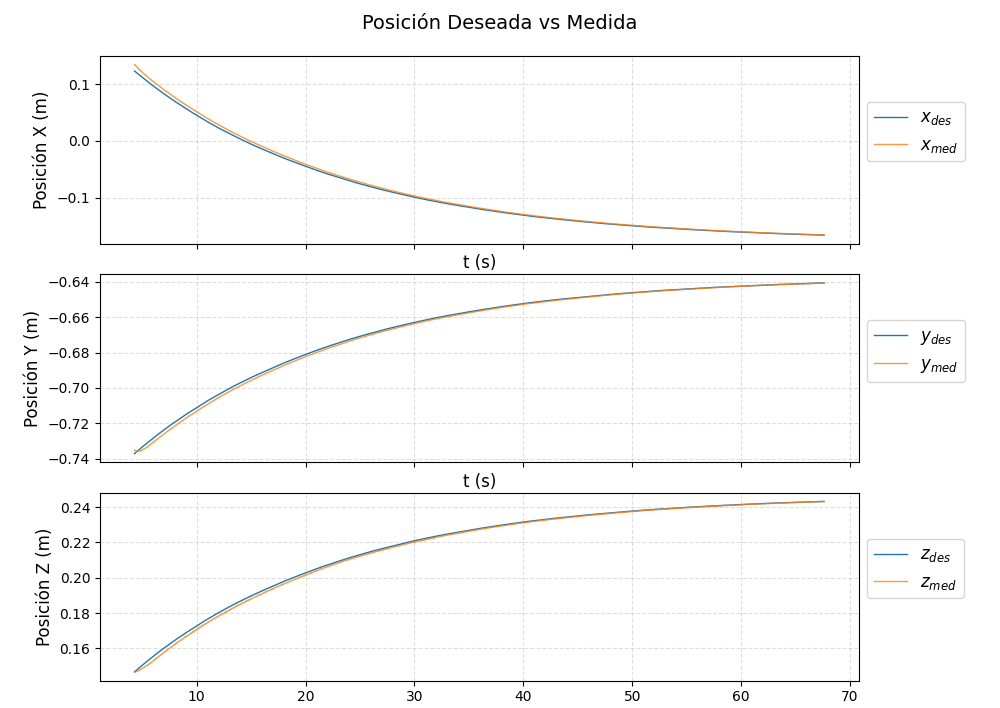
\includegraphics[width=0.75\linewidth]{images/Impedancia_XYZ_1.png}
    \caption{Seguimiento por eje cartesiano, control por impedancia, trayectoria recta}
    \label{fig:imp_recta_xyz}
\end{figure}

\begin{figure}[H]
    \centering
    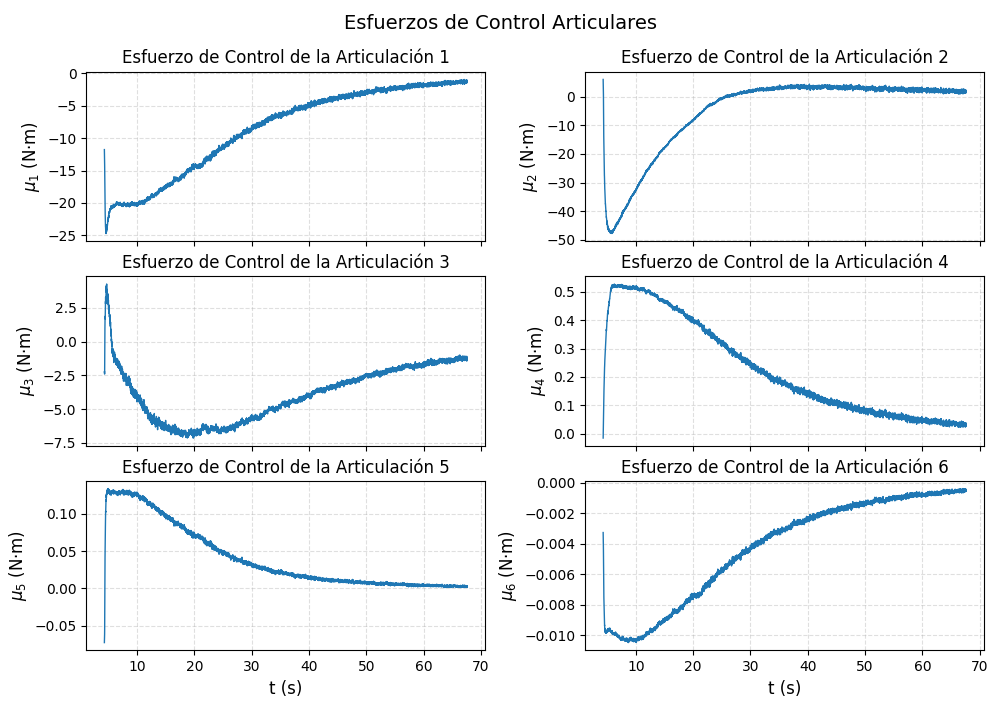
\includegraphics[width=1\linewidth]{images/Impedancia_u_1.png}
    \caption{Esfuerzo de control, control por impedancia, trayectoria recta}
    \label{fig:imp_recta_u}
\end{figure}

\begin{figure}[H]
    \centering
    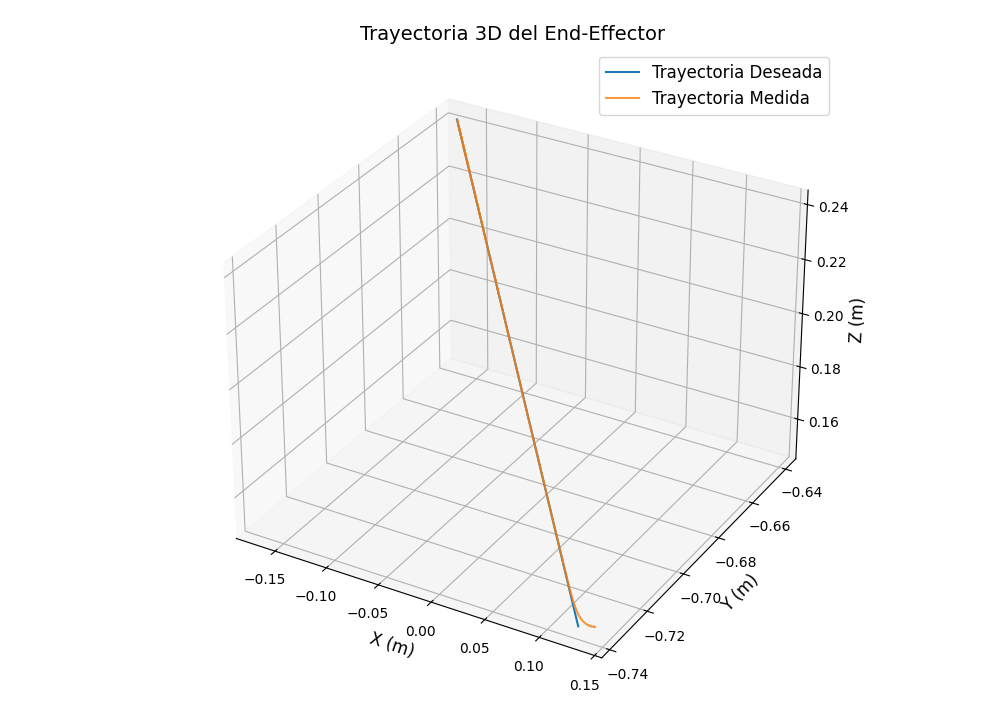
\includegraphics[width=1\linewidth]{images/Impedancia_3D_1.png}
    \caption{Seguimiento tridimensional, control por impedancia, trayectoria recta}
    \label{fig:imp_recta_3d}
\end{figure}

Sobre la trayectoria recta, el control por impedancia alcanzó un error de
posición máximo de $12.2$ mm (RMS $3.6$ mm), concentrado principalmente en el
eje $x$ (máximo $12.1$ mm), mientras que los ejes $y$ y $z$ se mantuvieron por
debajo de $2.7$ mm. El error de orientación se mantuvo por debajo de
$0.9^{\circ}$ durante toda la corrida.

\subsubsection{Curva helicoidal}

\begin{figure}[H]
    \centering
    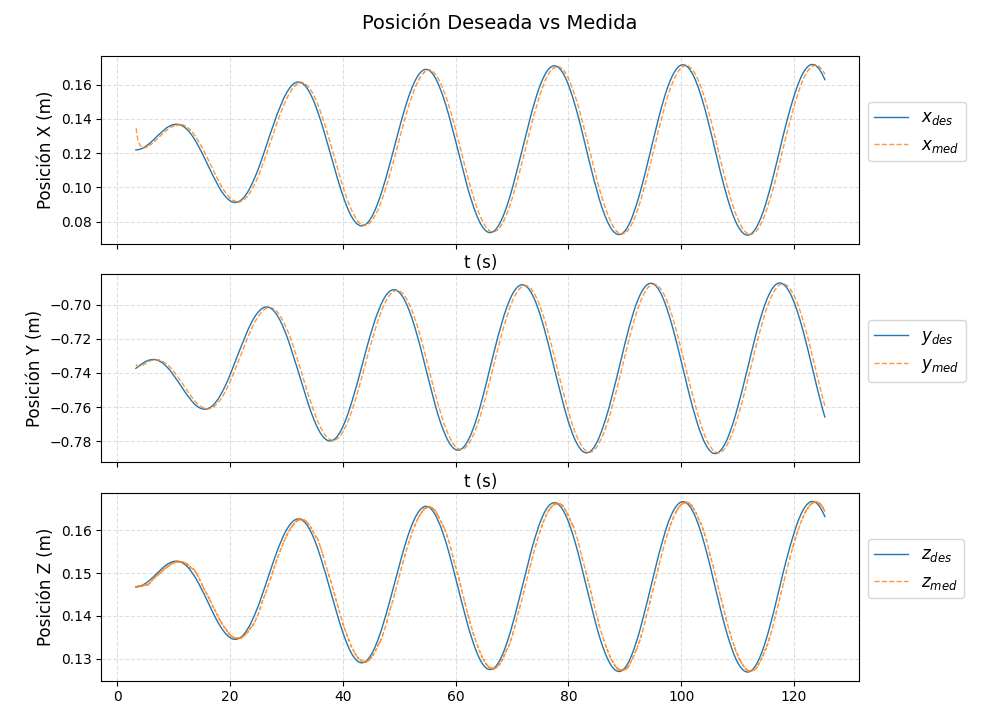
\includegraphics[width=0.75\linewidth]{images/Impedancia_XYZ_2.png}
    \caption{Seguimiento por eje cartesiano, control por impedancia, curva helicoidal}
    \label{fig:imp_heli_xyz}
\end{figure}

\begin{figure}[H]
    \centering
    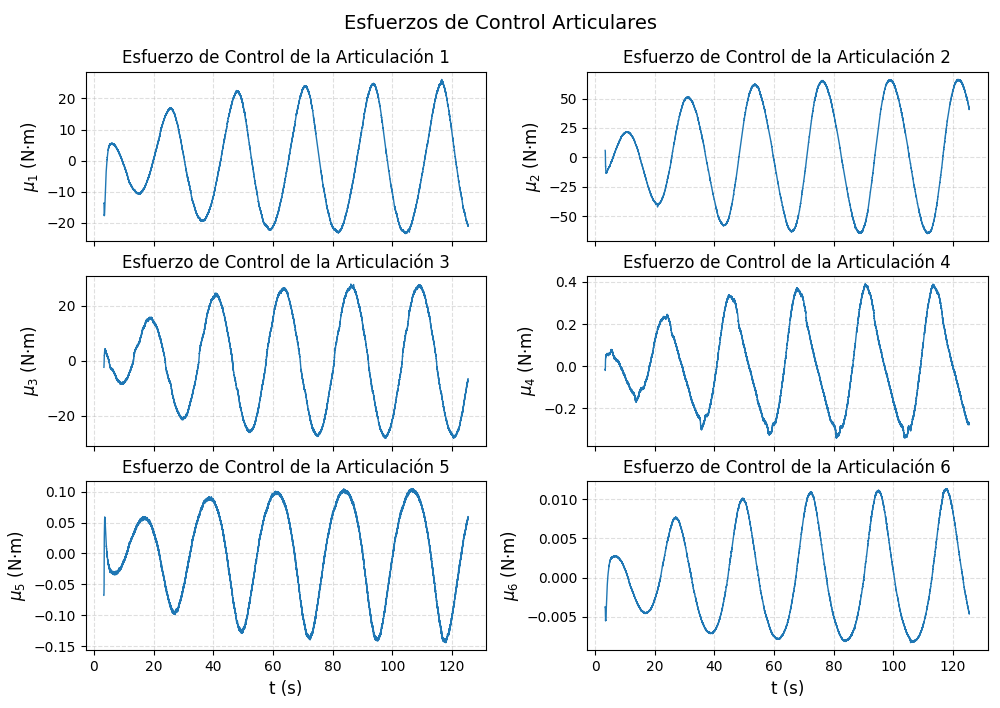
\includegraphics[width=1\linewidth]{images/Impedancia_u_2.png}
    \caption{Esfuerzo de control, control por impedancia, curva helicoidal}
    \label{fig:imp_heli_u}
\end{figure}

\begin{figure}[H]
    \centering
    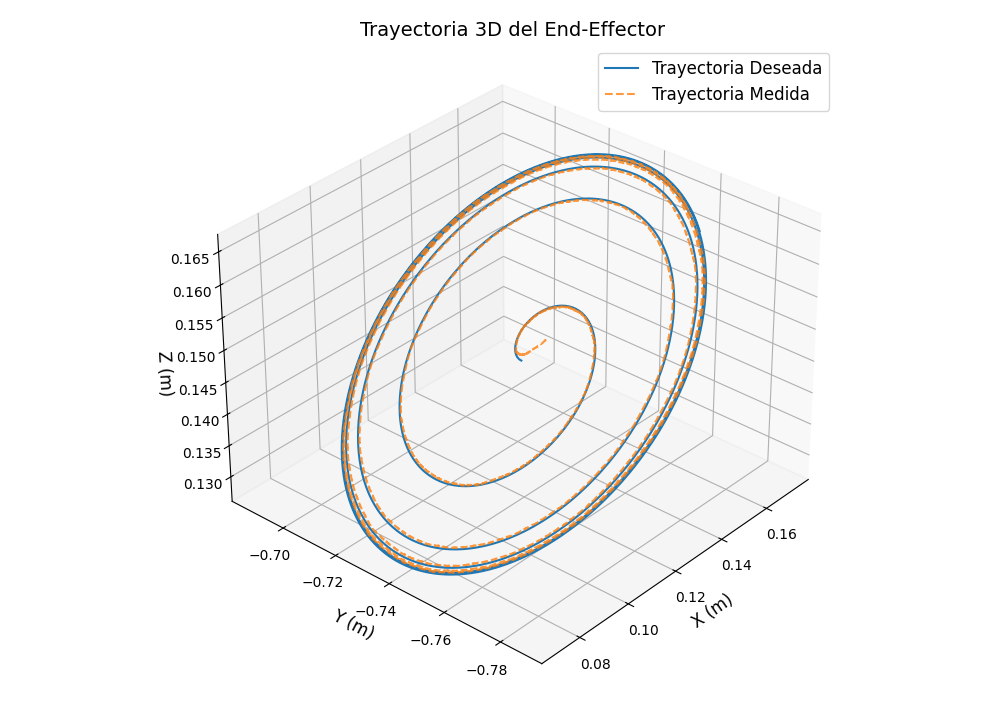
\includegraphics[width=1\linewidth]{images/Impedancia_3D_2.png}
    \caption{Seguimiento tridimensional, control por impedancia, curva helicoidal}
    \label{fig:imp_heli_3d}
\end{figure}

En la curva helicoidal, más exigente en aceleración y cambio de dirección, el
error máximo se mantuvo similar en magnitud ($12.8$ mm) pero el error RMS casi
se duplicó respecto a la trayectoria recta ($6.7$ mm), reflejando un error de
seguimiento sostenido en lugar de picos puntuales; el esfuerzo de control
promedio también aumentó considerablemente, de $13.7$ a $43.7$ (norma del
vector de torque registrado).

\subsection{Control por modo deslizante}

\subsubsection{Trayectoria recta}

\begin{figure}[H]
    \centering
    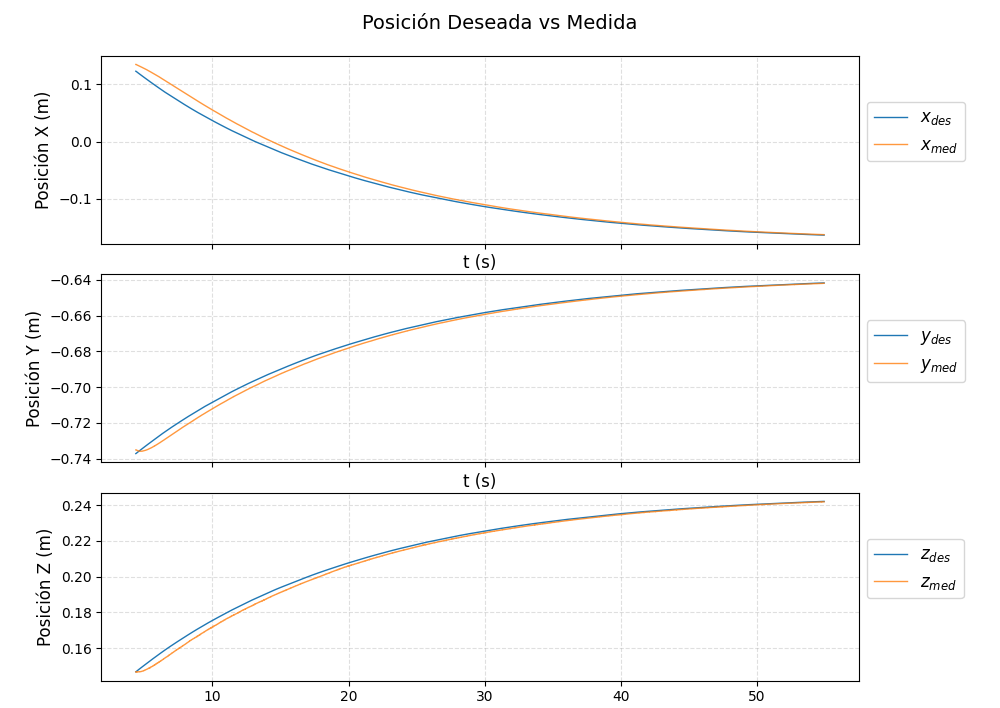
\includegraphics[width=0.75\linewidth]{images/Sliding_XYZ_1.png}
    \caption{Seguimiento por eje cartesiano, control por modo deslizante, trayectoria recta}
    \label{fig:sld_recta_xyz}
\end{figure}

\begin{figure}[H]
    \centering
    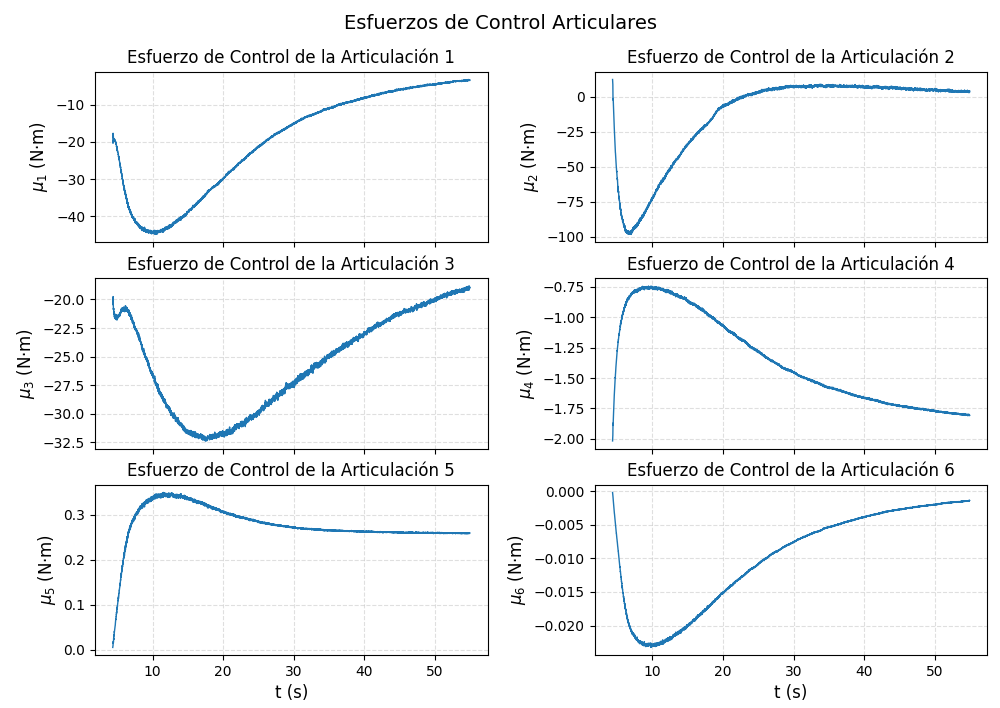
\includegraphics[width=1\linewidth]{images/Sliding_u_1.png}
    \caption{Esfuerzo de control, control por modo deslizante, trayectoria recta}
    \label{fig:sld_recta_u}
\end{figure}

\begin{figure}[H]
    \centering
    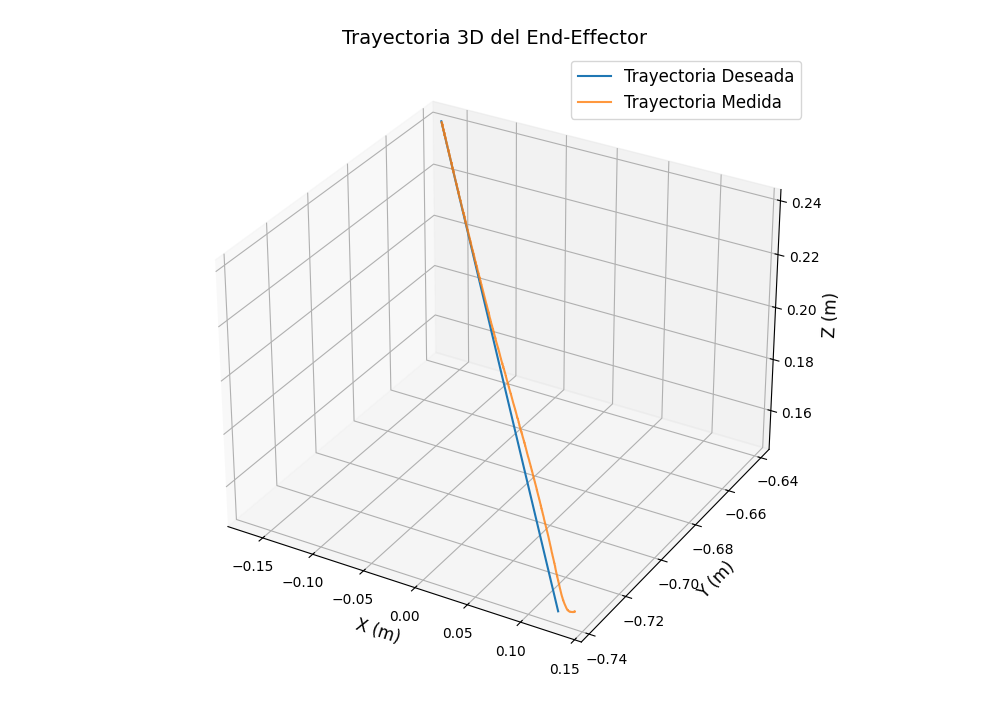
\includegraphics[width=1\linewidth]{images/Sliding_3D_1.png}
    \caption{Seguimiento tridimensional, control por modo deslizante, trayectoria recta}
    \label{fig:sld_recta_3d}
\end{figure}

El control por modo deslizante presentó el mayor error de seguimiento entre
las tres arquitecturas en la trayectoria recta, con un máximo de $21.6$ mm y
un RMS de $9.2$ mm, concentrado nuevamente en el eje $x$. El esfuerzo de
control promedio ($42.0$) resultó comparable al de impedancia en su corrida
más exigente, a pesar de tratarse aquí de la trayectoria más simple.

\subsubsection{Curva helicoidal}

\begin{figure}[H]
    \centering
    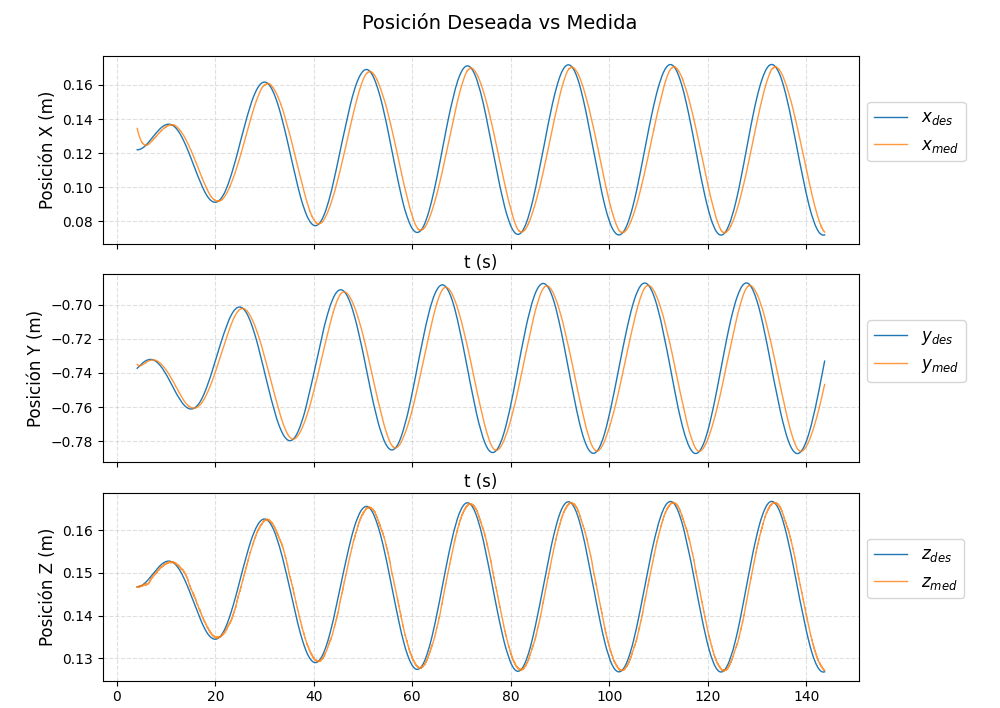
\includegraphics[width=0.75\linewidth]{images/Sliding_XYZ_2.png}
    \caption{Seguimiento por eje cartesiano, control por modo deslizante, curva helicoidal}
    \label{fig:sld_heli_xyz}
\end{figure}

\begin{figure}[H]
    \centering
    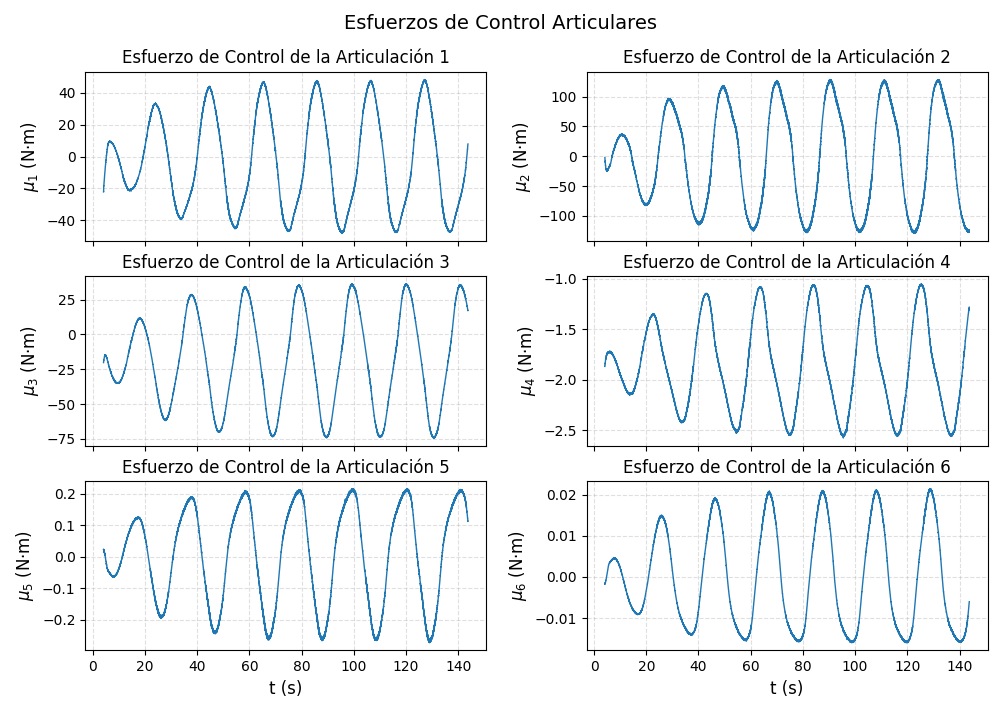
\includegraphics[width=1\linewidth]{images/Sliding_u_2.png}
    \caption{Esfuerzo de control, control por modo deslizante, curva helicoidal}
    \label{fig:sld_heli_u}
\end{figure}

\begin{figure}[H]
    \centering
    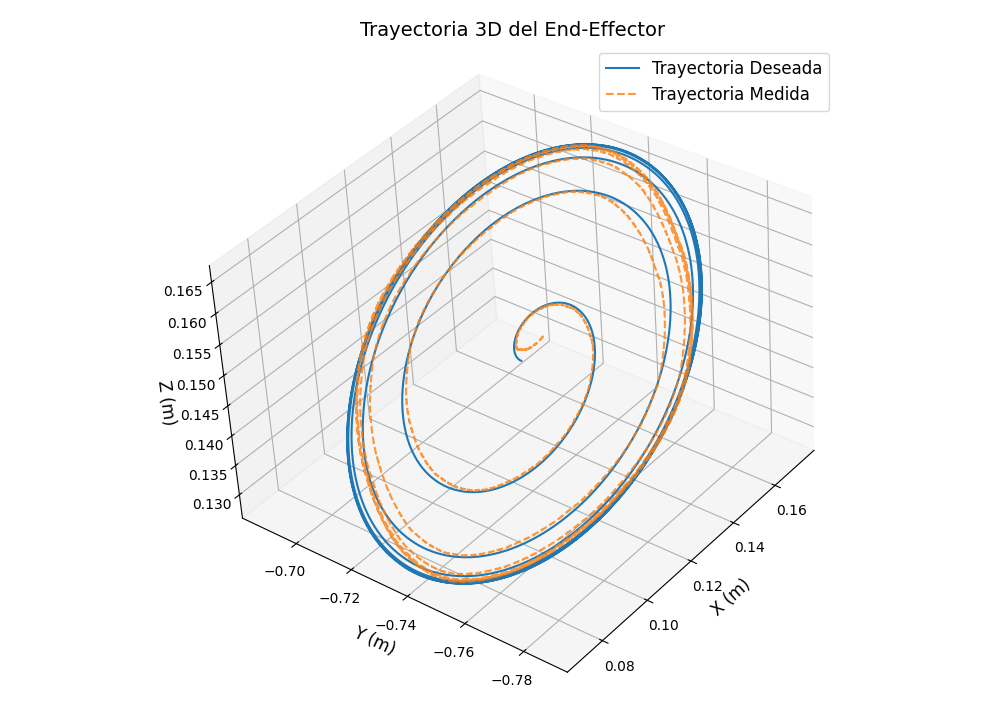
\includegraphics[width=1\linewidth]{images/Sliding_3D_2.png}
    \caption{Seguimiento tridimensional, control por modo deslizante, curva helicoidal}
    \label{fig:sld_heli_3d}
\end{figure}

En la curva helicoidal, el error RMS del SMC se elevó a $12.6$ mm, el más
alto de las seis corridas evaluadas, con el error prácticamente repartido por
igual entre los ejes $x$ y $y$ ($8.8$ mm RMS cada uno). El esfuerzo de control
promedio ($91.3$) también fue el más alto registrado, más del doble que en la
trayectoria recta, lo que sugiere que esta arquitectura, con las ganancias
utilizadas, tuvo mayor dificultad para adaptarse a los cambios de dirección
sostenidos de esta trayectoria.

\subsection{Optimización cuadrática (QP)}

\subsubsection{Trayectoria recta}

\begin{figure}[H]
    \centering
    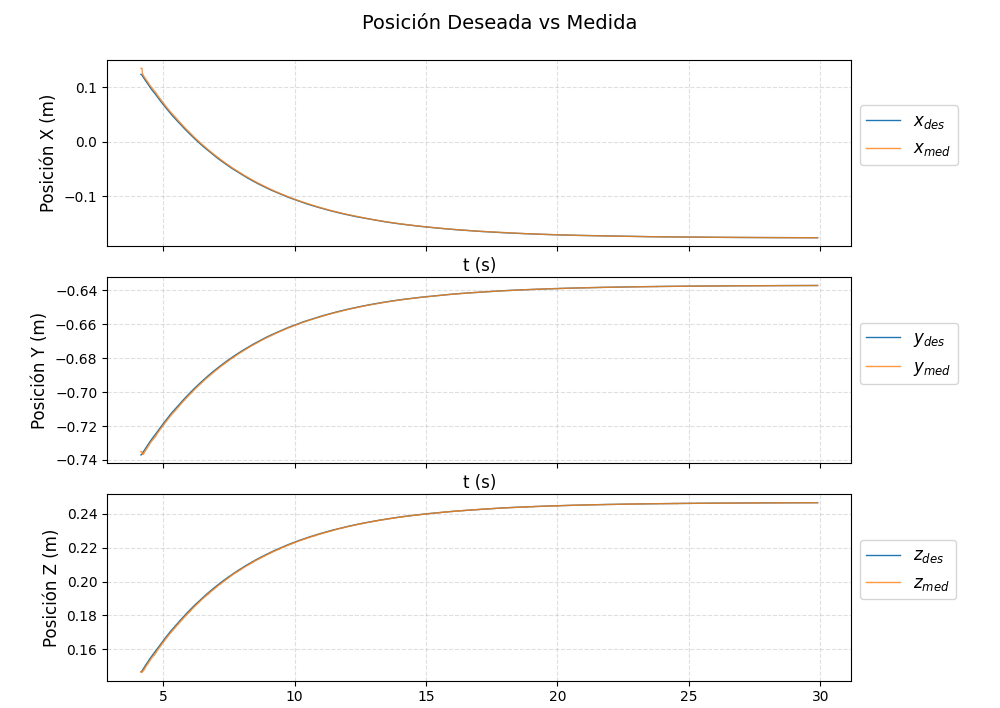
\includegraphics[width=0.75\linewidth]{images/QP_XYZ_1.png}
    \caption{Seguimiento por eje cartesiano, optimización cuadrática, trayectoria recta}
    \label{fig:qp_recta_xyz}
\end{figure}

\begin{figure}[H]
    \centering
    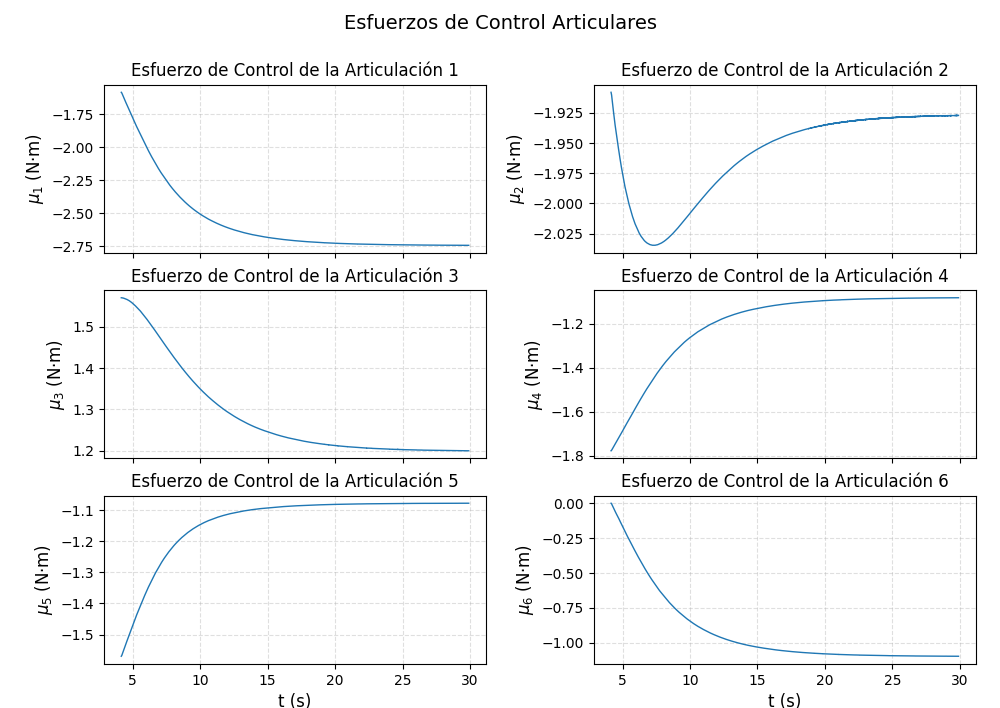
\includegraphics[width=1\linewidth]{images/QP_u_1.png}
    \caption{Esfuerzo de control, optimización cuadrática, trayectoria recta}
    \label{fig:qp_recta_u}
\end{figure}

\begin{figure}[H]
    \centering
    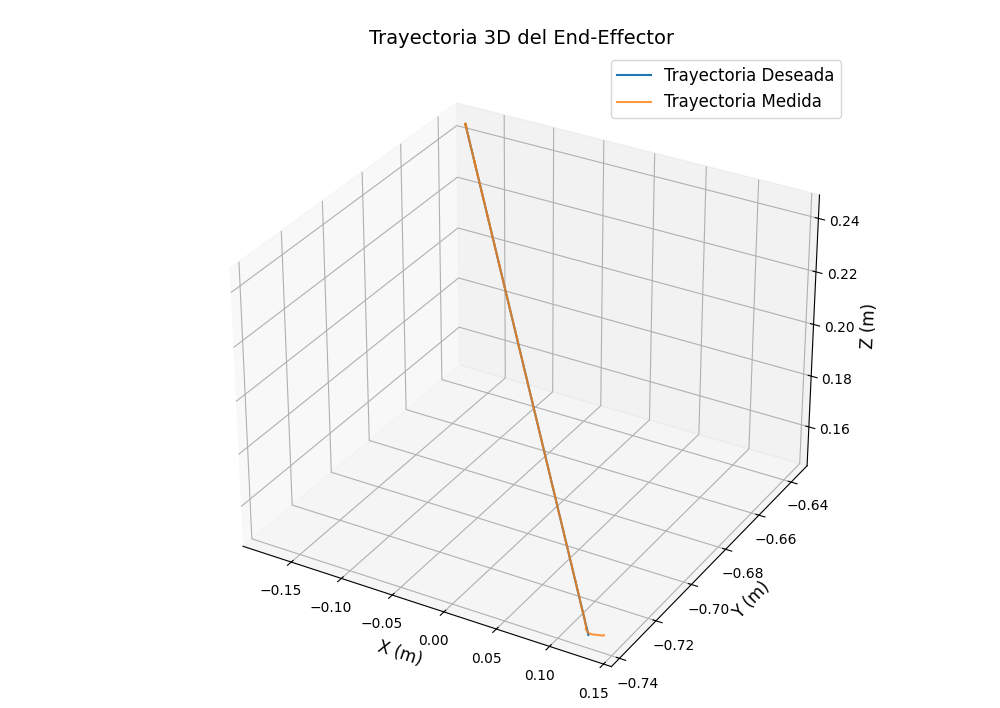
\includegraphics[width=1\linewidth]{images/QP_3D_1.png}
    \caption{Seguimiento tridimensional, optimización cuadrática, trayectoria recta}
    \label{fig:qp_recta_3d}
\end{figure}

El optimizador QP alcanzó un error máximo similar en magnitud a las otras dos
arquitecturas en el eje $x$ ($12.3$ mm, asociado al arranque de la
trayectoria), pero un error RMS notablemente menor ($1.2$ mm), casi un orden
de magnitud por debajo de impedancia y SMC. Cabe precisar que, al ser una
arquitectura puramente cinemática, el QP no calcula torque; el esfuerzo de
control aquí graficado corresponde al paso articular $\Delta q$ resuelto en
cada iteración, no a un par aplicado, por lo que no es directamente comparable
en magnitud con el de impedancia o SMC.

\subsubsection{Curva helicoidal}

\begin{figure}[H]
    \centering
    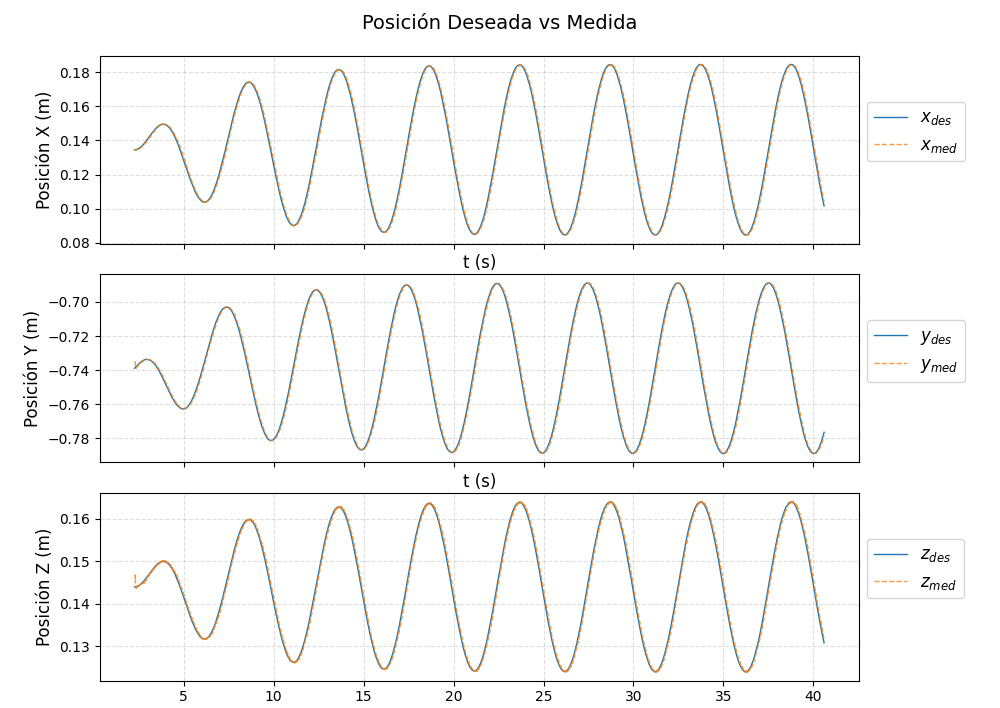
\includegraphics[width=0.75\linewidth]{images/QP_XYZ_2.png}
    \caption{Seguimiento por eje cartesiano, optimización cuadrática, curva helicoidal}
    \label{fig:qp_heli_xyz}
\end{figure}

\begin{figure}[H]
    \centering
    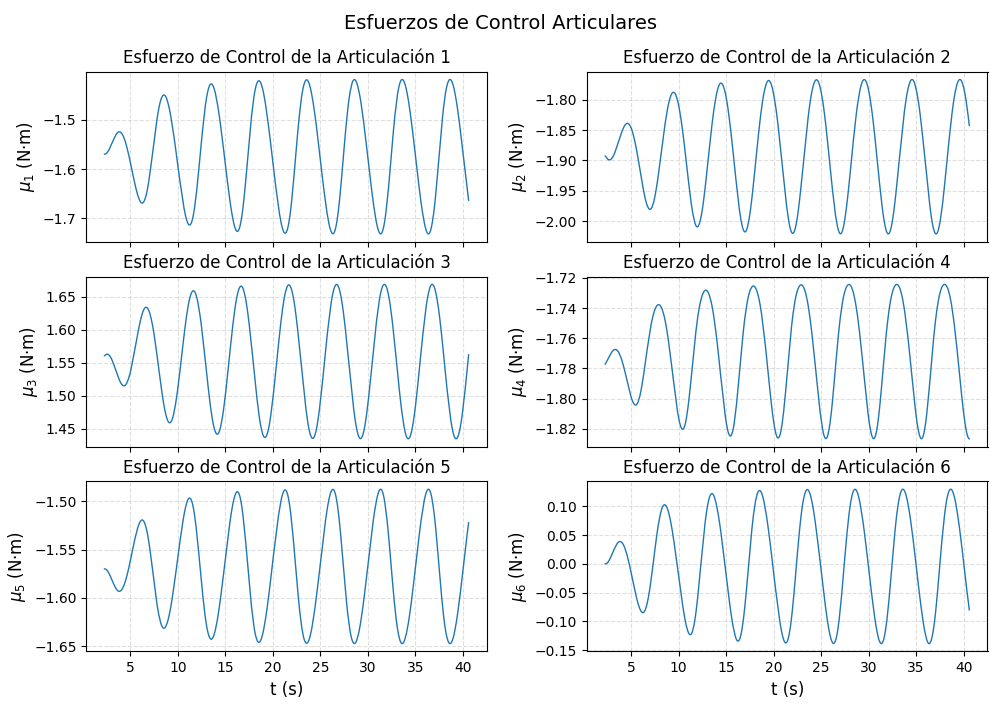
\includegraphics[width=1\linewidth]{images/QP_u_2.png}
    \caption{Esfuerzo de control, optimización cuadrática, curva helicoidal}
    \label{fig:qp_heli_u}
\end{figure}

\begin{figure}[H]
    \centering
    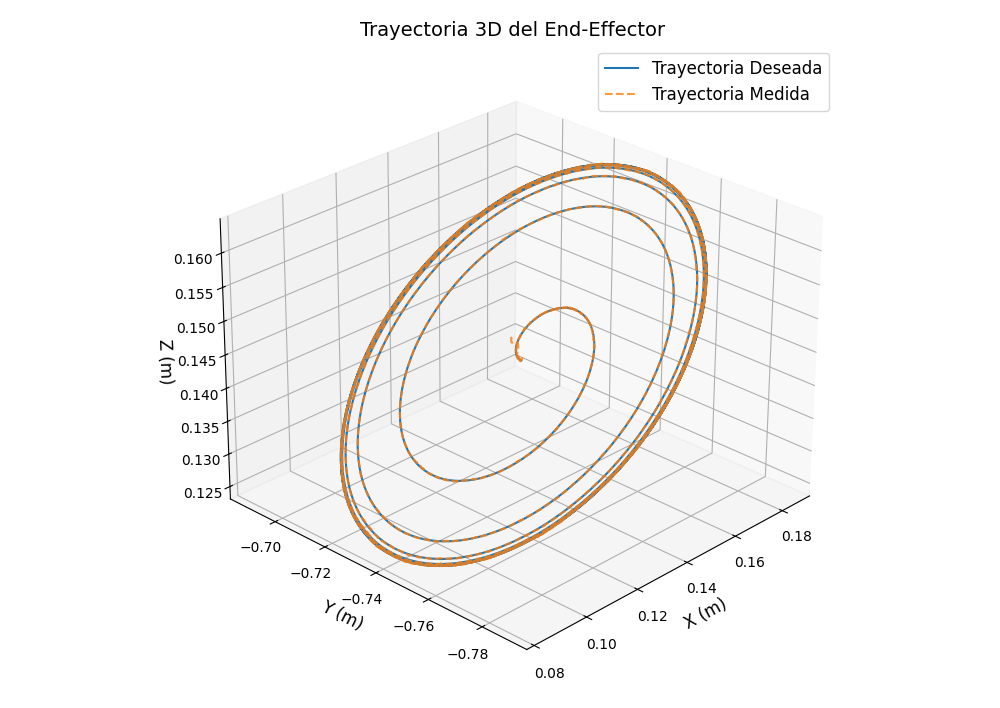
\includegraphics[width=1\linewidth]{images/QP_3D_2.png}
    \caption{Seguimiento tridimensional, optimización cuadrática, curva helicoidal}
    \label{fig:qp_heli_3d}
\end{figure}

En la curva helicoidal, el QP fue la única arquitectura cuyo error máximo se
redujo respecto a la trayectoria recta ($5.4$ mm) en lugar de mantenerse o
aumentar, con un RMS de $3.1$ mm. Esto sugiere que, a diferencia de los
controladores dinámicos, el desempeño del QP está menos condicionado por la
naturaleza de la trayectoria y más por el punto de arranque del seguimiento.

\subsection{Síntesis comparativa}

La Tabla \ref{tab:comparacion_arquitecturas} resume las métricas obtenidas en
las seis corridas evaluadas.

\begin{table}[H]
    \centering
    \begin{tabular}{l|c|c|c|c|c}
        \textbf{Arquitectura} & \textbf{Trayectoria} & \textbf{Err. máx. (mm)} & \textbf{Err. RMS (mm)} & \textbf{Esf. control prom.} & \textbf{Cómputo prom. (ms)} \\
        \hline
        Impedancia & Recta      & 12.2 & 3.6  & 13.7 & 9.2 \\
        Impedancia & Helicoidal & 12.8 & 6.7  & 43.7 & 8.8 \\
        SMC        & Recta      & 21.6 & 9.2  & 42.0 & 8.0 \\
        SMC        & Helicoidal & 15.7 & 12.6 & 91.3 & 8.0 \\
        QP         & Recta      & 12.4 & 1.2  & 4.0$^{*}$  & 1.4 \\
        QP         & Helicoidal & 5.4  & 3.1  & 3.7$^{*}$  & 1.6 \\
    \end{tabular}
    \caption{Comparación de métricas de seguimiento entre arquitecturas de
        control. ($^{*}$El esfuerzo de control del QP corresponde al paso
        articular $\Delta q$, no a un torque, y no es directamente comparable
        con impedancia o SMC.)}
    \label{tab:comparacion_arquitecturas}
\end{table}

De las tres arquitecturas evaluadas, el optimizador QP obtuvo consistentemente
el menor error RMS de seguimiento en ambas trayectorias y el menor tiempo de
cómputo por ciclo (en promedio $1.4$--$1.6$ ms, frente a $8$--$9$ ms de los
controladores dinámicos), lo que además le permitió operar a una frecuencia
de control efectiva considerablemente mayor. El control por impedancia
presentó el segundo mejor desempeño en seguimiento, mientras que el SMC, con
las ganancias empleadas, mostró el mayor error y el mayor esfuerzo de control
en ambas trayectorias, particularmente en la curva helicoidal. En conjunto,
estos resultados sustentan la selección del optimizador QP como la
arquitectura de control para la etapa de teleoperación.

\section{Validación de teleoperación}

Con la arquitectura de mejor desempeño (QP), se validó el sistema completo
mediante un ejercicio de teleoperación en el que el operador guio el efector
final del UR5 a través del Geomagic Touch.

\begin{figure}[H]
    \centering
    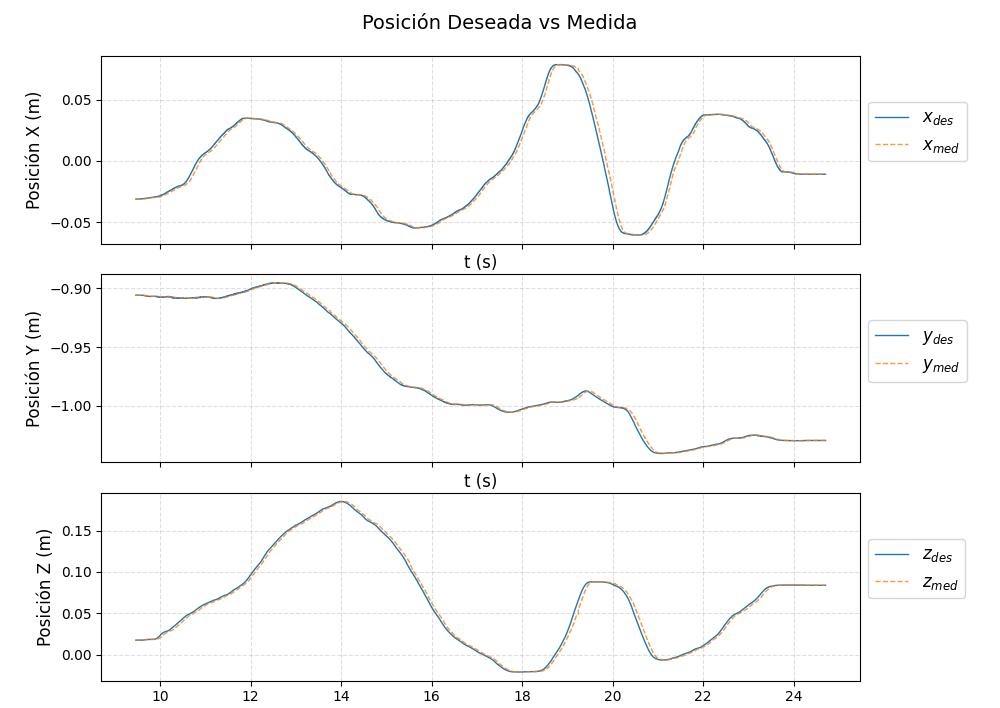
\includegraphics[width=0.75\linewidth]{images/QP_telop_XYZ.png}
    \caption{Seguimiento por eje cartesiano durante la teleoperación}
    \label{fig:qp_telop_xyz}
\end{figure}

\begin{figure}[H]
    \centering
    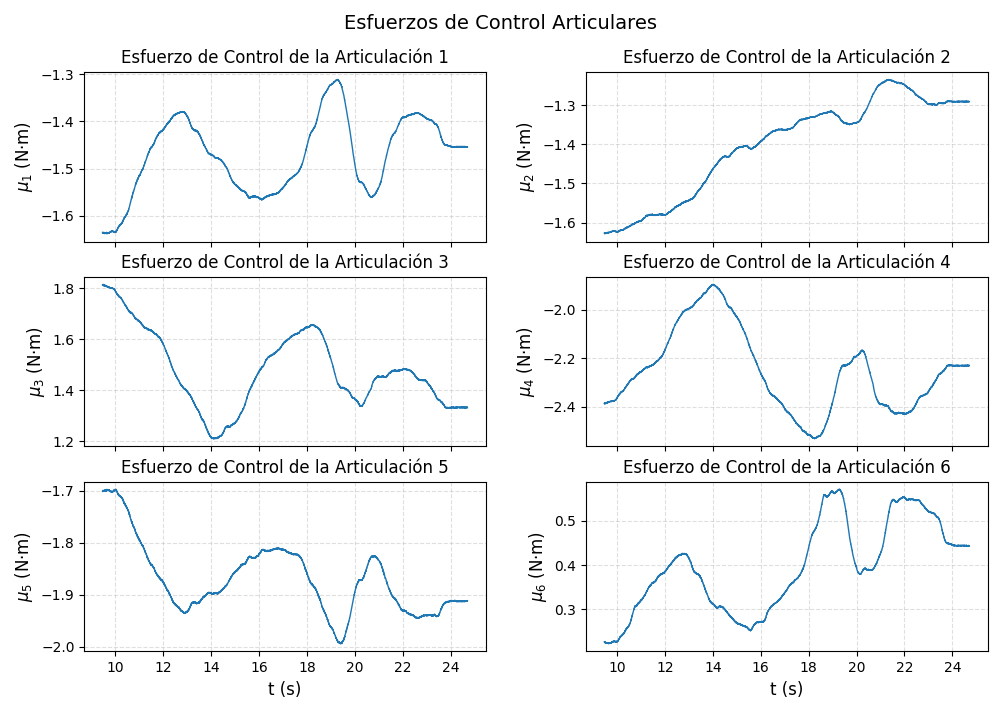
\includegraphics[width=1\linewidth]{images/QP_telop_u.png}
    \caption{Esfuerzo de control durante la teleoperación}
    \label{fig:qp_telop_u}
\end{figure}

\begin{figure}[H]
    \centering
    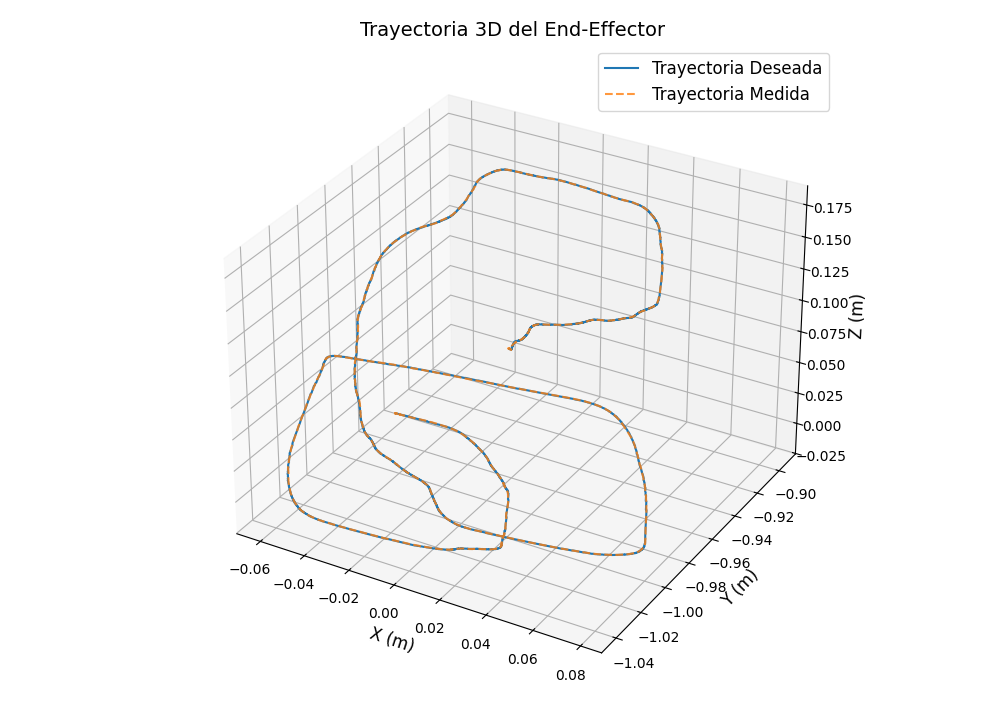
\includegraphics[width=1\linewidth]{images/QP_telop_3D.png}
    \caption{Seguimiento tridimensional durante la teleoperación}
    \label{fig:qp_telop_3d}
\end{figure}

Durante los $15.2$ s de la corrida, el error de posición se mantuvo con un
máximo de $18.3$ mm y un RMS de $5.1$ mm, en el mismo orden de magnitud que
las pruebas de seguimiento a trayectoria definida, a pesar de que aquí la
referencia es generada en tiempo real por el operador y no por una ecuación
suave predefinida. El registro de orientación de esta corrida muestra un
error angular anómalo (con valores cercanos a $180^{\circ}$) que no resulta
físicamente consistente con una teleoperación exitosa; esto indica muy
probablemente un problema en el cálculo del error de orientación (por
ejemplo, no elegir el sentido más corto de rotación entre cuaterniones
antípodas) y no un error real del efector final.
% Pendiente: revisar el cálculo de ori_err_angle en el nodo de control antes
% de reportar esta métrica en el cuerpo del texto o en una tabla.

\section{Validación con el banco de trabajo}

Finalmente, se evaluó el sistema integrado (teleoperación, control y
hardware) ejecutando una sutura sobre un kit de entrenamiento de cirugía
laparoscópica, empleando la arquitectura QP.
% Pendiente: esta sección aún no cuenta con registros CSV propios (a
% diferencia de las secciones anteriores). Completar con las métricas ya
% mencionadas en las Conclusiones (tiempo medio de sutura, error máximo de
% seguimiento, episodios de Jacobiano indeterminado) y, de ser posible, con
% figuras o datos del banco físico.
